\subsection{Aplicação Painel: Inserir}
\subsubsection*{Descrição do caso de uso}
Para inserir um registo, o utilizador necessita pressionar o botão \textit{Novo Registo}. A aparência da \textit{view} deste caso de utilização será semelhante ao demonstrado na figura \ref{fig:di_novo}. 

\begin{figure}[H] 
	\begin{center}
		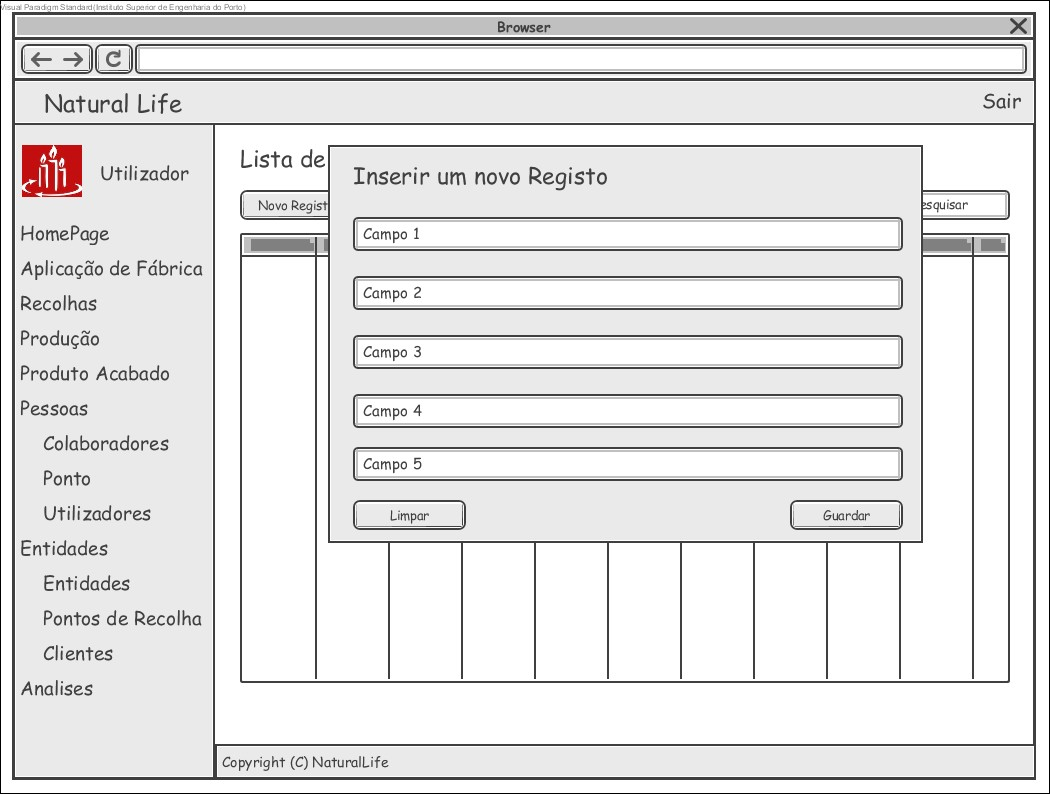
\includegraphics[width=0.60\textwidth,keepaspectratio]{figuras/Diagramas_vp/DI_Painel_2_Inserir.jpg}
		\caption{Modelo da janela de inserção na página de listagem}
		\label{fig:di_novo} 
	\end{center}
\end{figure}

\subsubsection*{\textit{Models} compatíveis com o caso de uso}
Todos os \textit{models} são compatíveis com este caso de uso

\subsubsection*{Fluxo do caso de utilização}
O caso de uso inicia-se quando o utilizador pressionar o botão novo registo na página de listagem. É apresentado uma janela flutuante com com os campos a serem preenchidos. O utilizador preenche os campos e pressiona o botão guardar. Finalizado o registo a janela fecha-se e é apresentado uma mensagem ao utilizador, tal como demonstrado na figura \ref{fig:sd_novo}.


\begin{figure}[H] 
	\begin{center}
		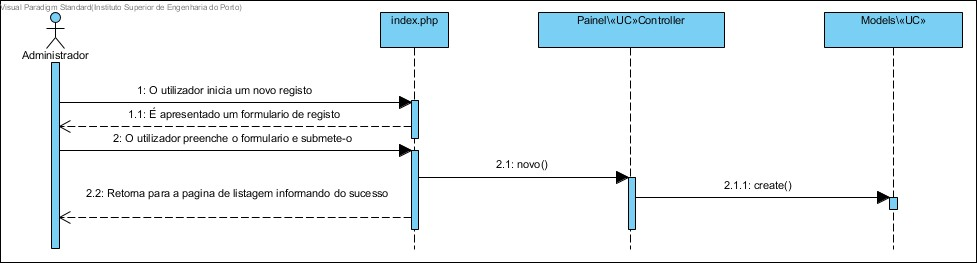
\includegraphics[width=\textwidth,keepaspectratio]{figuras/Diagramas_vp/SD_Painel_2_Inserir.jpg}
		\caption{Diagrama de sequência de inserir registo}
		\label{fig:sd_novo} 
	\end{center}
\end{figure}